\section{Bloczki procesu oraz start/end}
	Bloczek procesu jak nazwa wskazuje odpowiada za każdą akcje. W przypadku analizy kodu programistycznego bloczek ten odpowiada wywołaniu funkcji lub przypisaniu. Bloczek start/end w przypadku tej aplikacji od bloczka procesu różni się jedynie tym, że sygnalizuje on punkt startowy oraz wszystkie możliwe zakończenia algorytmu w danym schemacie. Aplikacja automatycznie zastępuje bloczki procesu występujące na początku i na końcu bloczkiem start/end. Dodatkowo aplikacja ignoruje wszystkie znaki typu $whitespace$ . Jeśli chcemy wprowadzić znak spacji do schematu należy użyć znaku "\_" (underscore), który zostanie zastąpiony. Aplikacja nie wymusza użycia elementów składniowych implikujących, że jest to wywołanie funkcji (zakończenie "...();") lub przypisanie (operator "="), do narysowania tego bloczku wymagane jest jedynie, by użyte były wyłącznie znaki należące do alfabetu w dowolnym języku (mające swój odpowiednik w Unicode),  
	
	\begin{figure}[H]
  \begin{subfigure}[t]{0.49\textwidth}
    \vspace{0pt}
    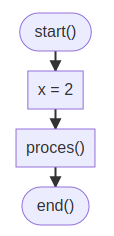
\includegraphics[height=6cm]{proces.png}
  \end{subfigure}\hfill
  \begin{subfigure}[t]{0.49\textwidth}
    \begin{minted}[linenos=true]{cpp}
start();
x _ = _ 2;
proces();
end();
    \end{minted}
  \end{subfigure}%
  \caption{Bloczki procesu, start/end wraz z kodem, który je generuje}
\end{figure}

\section{Bloczek warunkowy}
\begin{itemize}
	\item dla instrukcji $if-else$: {\smallskip}
	
		Aplikacja rozpoznaje składnie instrukcji i z podanego warunku tworzy bloczek decyzyjny. Następnie tworzy dwa rozgałęzienia odpowiadające za akcje (dowolna ilość bloczków procesu) wykonywane w przypadku spełnienia warunku (bezpośrednio pod scope'm intrukcji $if$) lub nie spełnienia (pod scope'm instrukcji $else$, a następnie instrukcje znajujące się poza intrukcją $if$) 
		
			\begin{figure}[H]
  \begin{subfigure}[t]{0.49\textwidth}
    \vspace{0pt}
    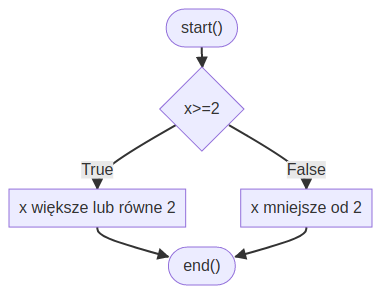
\includegraphics[height=6cm]{decyzja-if.png}
  \end{subfigure}\hfill
  \begin{subfigure}[t]{0.44\textwidth}
    \begin{minted}[linenos=true]{cpp}
start();
if(x >= 2){
  x_większe_lub_równe_2;
}
else{
  x_mniejsze_od_2;
}
end();
    \end{minted}
  \end{subfigure}%
  \caption{Bloczek warunkowy utworzony przy użyciu instrukcji $if$}
\end{figure}
	
	\item dla instrukcji $while$: {\smallskip}
	
		Interpretacja warunku działa analogicznie jak przy instrukcji $if$, podobnie również działa dołączanie kolejnych instrukcji wykonujących się po spełnieniu warunku z tą różnicą, że ostatni proces tej gałęzi łączony jest automatycznie z bloczkiem decyzyjnym instrukcji $while$. Nie spełnienie warunku odpowiada gałęzi na której znajdują się procesy umieszczone poza scope'm  tego typu instrukcji warunkowej.
	
				\begin{figure}[H]
  \begin{subfigure}[t]{0.49\textwidth}
    \vspace{0pt}
    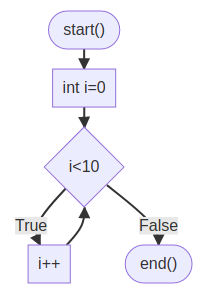
\includegraphics[height=6cm]{decyzja-while.png}
  \end{subfigure}\hfill
  \begin{subfigure}[t]{0.44\textwidth}
    \begin{minted}[linenos=true]{cpp}
start();
int_ i = 0;
while(i < 10){
  i++;
}
end();
    \end{minted}
  \end{subfigure}%
  \caption{Bloczek warunkowy utworzony przy użyciu instrukcji $while$}
\end{figure}	
		
\end{itemize}

\section{Bardziej złożony przykład}
Schemat blokowy przedstawiający (uproszczony) algorytm działania aplikacji w której został narysowany: {\smallskip}

			\begin{figure}[H]
  \begin{subfigure}{\textwidth}
    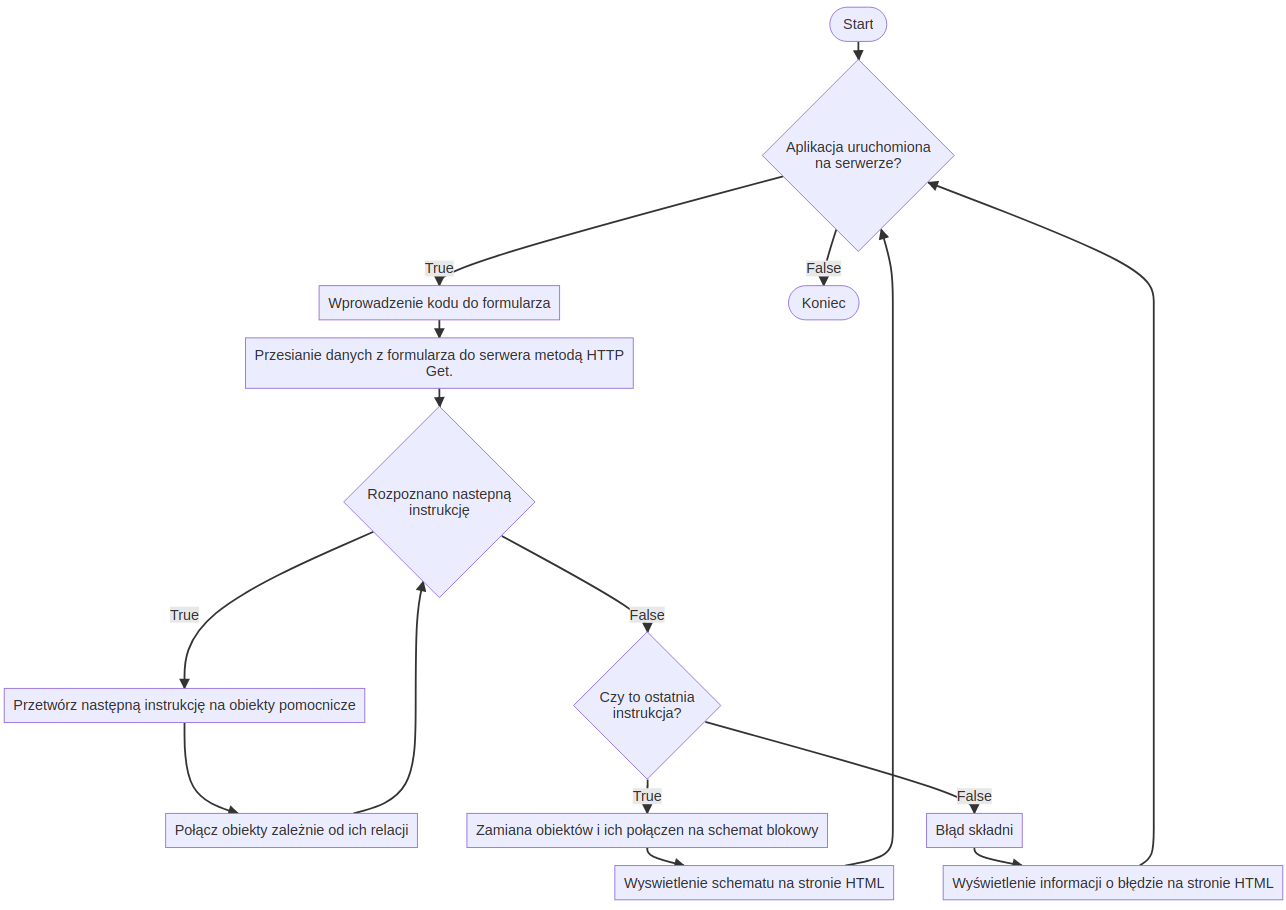
\includegraphics[width=\textwidth]{aplikacja-flowchart.png}
  \end{subfigure}\hfill
  \begin{subfigure}[t]{0.44\textwidth}
    \begin{minted}[linenos=true]{cpp}
Start;
while(Aplikacja _ uruchomiona _ na _ serwerze?){
    Wprowadzenie_ kodu_ do_ formularza;
    Przesianie_ danych_ z_ formularza_ do_ serwera_ metodą_ HTTP_ Get.;
    while(Rozpoznano_ nastepną_ instrukcję){
        Przetwórz_ następną_ instrukcję_ na_ obiekty_ pomocnicze;
        Połącz_ obiekty_ zależnie_ od_ ich_ relacji;
    }
    if(Czy_ to_ ostatnia_ instrukcja?){
    Zamiana_ obiektów_ i_ ich_ połączeń_ na_ schemat_ blokowy;
    Wyswietlenie _ schematu _ na _ stronie _ HTML;
    } else {
        Błąd _ składni;
        Wyświetlenie _ informacji _ o _ błędzie _ na _ stronie _ HTML;
    }
}
Koniec;
    \end{minted}
  \end{subfigure}%
  \caption{Przykład pokazujący obsługę zagnieżdżonych instrukcji warunkowych, zawijanie tekstu oraz wprowadzanie polskich znaków}
\end{figure}